\documentclass{beamer}

\title{Reinforcement Learning for the Asymmetric Traveling Salesperson Problem with Precedence Constraints}
\author{Elisabeth Bankl}
\date{\today}

\begin{document}

\frame{\titlepage}



\begin{frame}
    \frametitle{Problem Statement 1}
    \begin{itemize}
        \item A set of tasks that need to be completed after another
        \item Some tasks need to be finished before starting others (precedence constraints)
        \item The execution time of a task depends on the task before it (transition time)
        \item Objective: Find the best order to execute the tasks that minimizes the total execution time and follows all precedence constraints
        \item Asymmetric Travelling Salesperson Problem with Precedence Constraints: nodes represent tasks, distances represent transition times
    \end{itemize}
   

\end{frame}

\begin{frame}
    \frametitle{Problem Statement 1}
    \begin{figure}
        \centering
        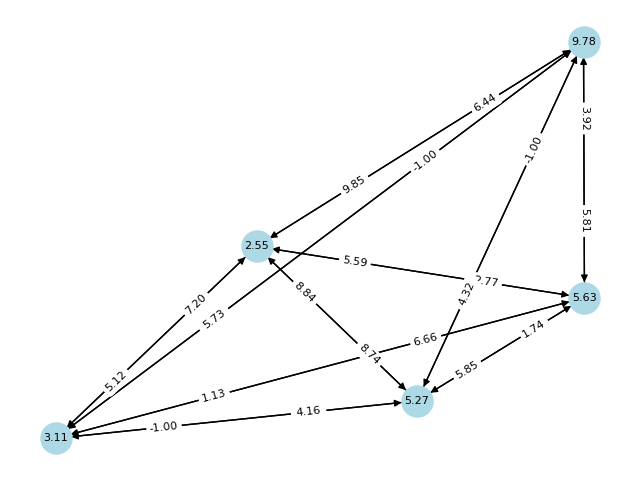
\includegraphics[width=0.8\textwidth]{graph_visualization.png}
        \caption{Graph visualization of the problem}
    \end{figure}

\end{frame}


\begin{frame}
    \frametitle{MDP Formulation}
    \begin{itemize}
        \item \textbf{State Space}: The state includes:
        \begin{itemize}
            \item \textbf{Distance Matrix (D)}: Represents the distances between nodes.
            \item \textbf{Precedence Matrix (P)}: Indicates which nodes must be visited before others.
            \item \textbf{Cost Matrix (C)}: Contains the cost of starting at a node and the cost of traveling between nodes.
            \item \textbf{Visited Nodes Vector (V)}: A binary vector indicating which nodes have been visited.
        \end{itemize}
        \item \textbf{Action Space}: The actions are the nodes that the agent can visit next. However, actions are restricted:
        \begin{itemize}
            \item Nodes with unfulfilled precedence constraints are not allowed.
            \item Nodes that have already been visited are not allowed.
        \end{itemize}
        \item \textbf{Reward Function}: The reward is calculated based on the action taken:
        \begin{itemize}
            \item If the action violates precedence constraints, a large negative reward is given.
            \item If the action is valid, the reward is the negative of the distance between the current node and new node.
        \end{itemize}
    \end{itemize}
\end{frame}

\begin{frame}
    \frametitle{Reinforcement Learning Algorithm}
    \begin{itemize}
        \item \textbf{Algorithm}: Proximal Policy Optimization (PPO)
        \item \textbf{Network Architecture}: MLP
    \end{itemize}
\end{frame}

\begin{frame}
    \frametitle{Dataset}
    \begin{itemize}
        \item Problem instances randomly generated during training
        \item Randomly sample distances between nodes, precedence constraints and node costs
    \end{itemize}
\end{frame}


\begin{frame}
    \frametitle{Reward Curve for RL Agent}
    \begin{figure}
        \centering
        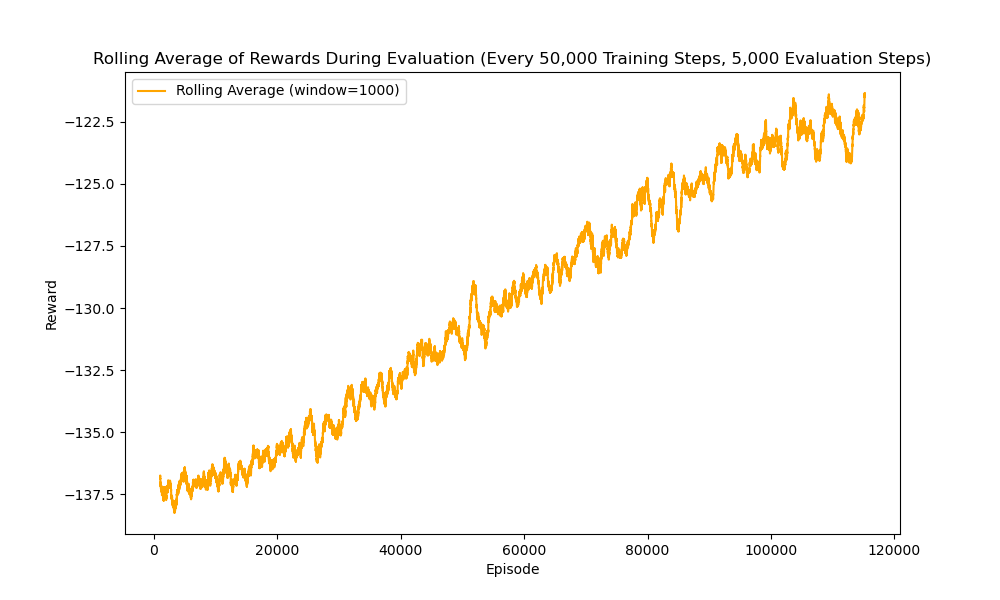
\includegraphics[width=0.8\textwidth]{reward_trajectory.png}
        \caption{Reward curve for the reinforcement learning agent during training}
    \end{figure}
\end{frame}

\begin{frame}
    \frametitle{Comparison with simple algorithms}
    \begin{table}[]
        \centering
        \begin{tabular}{|c|c|}
            \hline
            \textbf{Algorithm} & \textbf{Average Reward} \\
            \hline
            Random Algorithm & -137.5 \\  % Corrected typo: "Randomn" to "Random"
            \hline
            Greedy Algorithm & -85 \\
            \hline
            Reinforcement Learning Agent & -123 \\
            \hline
        \end{tabular}
        \caption{Performance comparison of different algorithms}
    \end{table}
\end{frame}

\end{document}